\documentclass[12pt, a4paper]{article} % book, report, article, letter, slides
                                       % letterpaper/a4paper, 10pt/11pt/12pt, twocolumn/twoside/landscape/draft

%%%%%%%%%%%%%%%% PACKAGES %%%%%%%%%%%%%%%%%%%%%

\usepackage[utf8]{inputenc} % encoding

\usepackage[english]{babel} % use special characters and also translates some elements within the document.

\usepackage{amsmath}        % Math
\usepackage{amssymb}        % Math, extended collection
\usepackage{amsthm}         % Math, \newtheorem, \proof, etc
\newtheorem{theorem}{Theorem}[section]
\newtheorem{corollary}{Corollary}[theorem]
\newtheorem{lemma}[theorem]{Lemma}


\usepackage{hyperref}       % Hyperlinks \url{url} or \href{url}{name}

\usepackage{parskip}        % \par starts on left (not idented)

\usepackage{abstract}       % Abstract

\usepackage{tocbibind}      % Adds the bibliography to the table of contents (automatically)

\usepackage{graphicx}       % Images
\graphicspath{ {./images/} }

% \usepackage[document]{ragged2e}  % Left-aligned (whole document)
% \begin{...} ... \end{...}   flushleft, flushright, center

%%%%%%%%%%%%%%%% GRAPHICS %%%%%%%%%%%%%%%%%%%%%

\usepackage{tikz}
\usetikzlibrary{arrows}

\tikzset{
  treenode/.style = {align=center, inner sep=0pt, text centered,
    font=\sffamily},
  arn_n/.style = {treenode, circle, white, font=\sffamily\bfseries, draw=black,
    fill=black, text width=1.5em},% arbre rouge noir, noeud noir
  arn_r/.style = {treenode, circle, red, draw=red,
    text width=1.5em, very thick},% arbre rouge noir, noeud rouge
  arn_x/.style = {treenode, rectangle, draw=black,
    minimum width=0.5em, minimum height=0.5em}% arbre rouge noir, nil
}

%%%%%%%%%%%%%%%% CODE %%%%%%%%%%%%%%%%%%%%%

\usepackage{minted}         % Code listing
% \mint{html}|<h2>Something <b>here</b></h2>|
% \inputminted{octave}{BitXorMatrix.m}

%\begin{listing}[H]
  %\begin{minted}[xleftmargin=20pt,linenos,bgcolor=codegray]{haskell}
  %\end{minted}
  %\caption{Example of a listing.}
  %\label{lst:example} % You can reference it by \ref{lst:example}
%\end{listing}

\newcommand{\code}[1]{\texttt{#1}} % Define \code{foo.hs} environment

%%%%%%%%%%%%%%%% COLOURS %%%%%%%%%%%%%%%%%%%%%

\usepackage{xcolor}         % Colours \definecolor, \color{codegray}
\definecolor{codegray}{rgb}{0.9, 0.9, 0.9}
% \color{codegray} ... ...
% \textcolor{red}{easily}

%%%%%%%%%%%%%%%% CONFIG %%%%%%%%%%%%%%%%%%%%%

\renewcommand{\absnamepos}{flushleft}
\setlength{\absleftindent}{0pt}
\setlength{\absrightindent}{0pt}

%%%%%%%%%%%%%%%% GLOSSARIES %%%%%%%%%%%%%%%%%%%%%

%\usepackage{glossaries}

%\makeglossaries % before entries

%\newglossaryentry{latex}{
    %name=latex,
    %description={Is a mark up language specially suited
    %for scientific documents}
%}

% Referene to a glossary \gls{latex}
% Print glossaries \printglossaries

%%%%%%%%%%%%%%%% HEADER %%%%%%%%%%%%%%%%%%%%%

\usepackage{fancyhdr}
\pagestyle{fancy}
\fancyhf{}
\rhead{Arnau Abella - MIRI}
\lhead{ADS - First Delivery}
\rfoot{Page \thepage}

%%%%%%%%%%%%%%%% TITLE %%%%%%%%%%%%%%%%%%%%%

\title{Red-black Trees: A Pure Functional Implementation}
\author{Arnau Abella}
\date{\today}

%%%%%%%%%%%%%%%% DOCUMENT %%%%%%%%%%%%%%%%%%%%%

\begin{document}

\maketitle

\section{Introduction}\label{s:introduction}

Although binary search trees work very well on random or unordered data, they perform very poorly on ordered data, for which any individual operation migh take up to $\mathcal{O}(n)$ time.

The solution to this problem is to keep each tree approximately balanced. Then no individual operation takes more than $\mathcal{O}(log n)$ time. There are several implementations of self-balancing binary search trees such as \textit{2-3 tree, AA tree, AVL tree, B-tree, Treap, etc}.

This delivery is about one of the most popular families of self-balancing binary search trees, the \textit{red-black trees} \cite{gs78}.

A \textbf{red-black tree} is a binary search tree in which every node is colored either red or black.

\begin{figure}[b]
  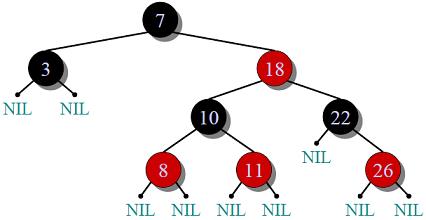
\includegraphics[scale=0.5]{rbt}
  \centering
  \caption{Example of a red-black tree.}
  \label{fig:rbt}
\end{figure}

Every red-black tree satisfy the following two balance invariants:

\begin{enumerate}
  \item No red node has a red child. \label{inv1}
  \item Every path from the root to an empty node contains the same number of black nodes. \label{inv2}
\end{enumerate}

Taken together, these two invariants guarantee that the longest possible path in a red-black tree, one with alternating black and red nodes, is no more than twice as long as the sorthest possible, one with black nodes only.

\begin{theorem}\label{t:balance}
  The maximum depth of a node in a red-black tree of size $n$ is at most $2\lfloor \log (n+1) \rfloor$
\end{theorem}

\begin{proof}\label{p:balance}
  The maximum number of black nodes in the longest path from the root to a leaf is restricted by the number of nodes in the shortest past (inv. \ref{inv2}).

  Assume that the shortest path has depth $k$. Then, there are $k+1$ nodes in a path of depth $k$.

  From the definition of the shortest path, there is a full and complete binary subtree of depth $k$ (that includes the shortest path). Suposse that the complete binary subtree has $n$ nodes. So, by the definition of a complete binary tree, $n = 2^{k+1} -1$. Hence, we can compute the number of nodes in the shortest by using the previous equation.

  \begin{align*}
    n     &= n^{k+1}-1 \\
    k + 1 &= \log_2 (n+1)
  \end{align*}

  The number f nodes in the shortest path is $\log_2 (n+1)$. So, the largest path can have, at most, $\log_2 (n+1)$ black nodes (inv. \ref{inv2}).

  Let's make the largest path with $\log_2 (n+1)$ black nodes. We want to put as many red nodes as possible because we are limited in the number of black nodes. But, because of the inv. \ref{inv1}, we need to alternate between black and red nodes.

  If the root is black, there will be as many red nodes as black ones. The depth $k$ of the largest path is the following:

  \begin{align*}
    k &= \#red \cdot \#black \\
    k &= \log_2 (n+1) \cdot \log_2 (n+1) \\
    k &= 2\lfloor \log_2 (n+1) \rfloor \\
    k &= \mathcal{O}(\log n)
  \end{align*}

\end{proof}

\section{Implementation}\label{s:implementation}

The implementation proposed in this first delivery for the \textbf{red-black tree} is a persistent representation written in \textbf{haskell} \cite{haskell}, an advanced, lazy, purely functional programming language, and based on the implementation from \textit{C. Okasaki} written in \textit{Standard ML} \cite{oka98}.

The proposed implementation has some tweaks $wrt.$ the implementation from \textit{C. Okasaki} that improve insertion time. Also, the implementation includes an auxiliar method to construct the \textit{red-black tree} in $\mathcal{O}(n)$ instead of $\mathcal{O}(n \log n)$.

The source code, that can be found in the \nameref{s:appendix-a}.

Let's have a look at the most interesting parts of the code. First, we will start with the data definition at listing \ref{lst:constructor}, which is pretty straightforward. I included some useful classes instances such as \code{functor, foldable and traversable}. The attentive readers will notice the exclamation marks in front of the data constructors. This is a language extension called \textit{BangPatterns} that allows changing how an expression is evaluated in haskell.

\begin{listing}[H]
  \begin{minted}[xleftmargin=20pt,linenos]{haskell}
data Color = R -- ^ Red
           | B -- ^ Black
  deriving (Show, Enum)

data RedBlackTree a
  = Bin Color !(RedBlackTree a) !a !(RedBlackTree a)
  | Tip
  deriving (Functor, Foldable, Traversable)
  \end{minted}
  \caption{Red-black tree data types}
  \label{lst:constructor}
\end{listing}

\newpage

The next method we are going to have a look into detail is \code{insert}. Insert is the hardest method to implement because it must not violate any of the two invariants after the insertion.

To not violate invariant \ref{inv2} we are going to always insert a \textbf{red} node but this may have broken the invariant \ref{inv1} if the parent was already red so we need to rebalance the tree, recursively.

Figure \ref{fig:violations} displays all possible configurations where the invariant 1 is violated.

\begin{figure}
\centering
    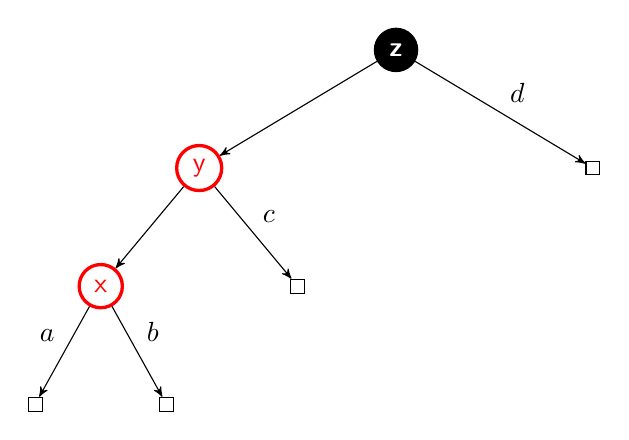
\begin{tikzpicture}[->,>=stealth',level/.style={sibling distance = 5cm/#1,level distance = 1.5cm}]
    \node [arn_n] {z}
        child{ node [arn_r] {y}
                child{ node [arn_r] {x}
                  child{ node [arn_x] {} edge from parent node[above left] {$a$}}
                  child{ node [arn_x] {} edge from parent node[above right] {$b$}}
                }
                child{ node [arn_x] {} edge from parent node[above right] {$c$}}
        }
        child{ node [arn_x] {} edge from parent node[above right] {$d$}}
    ;
    \end{tikzpicture}
    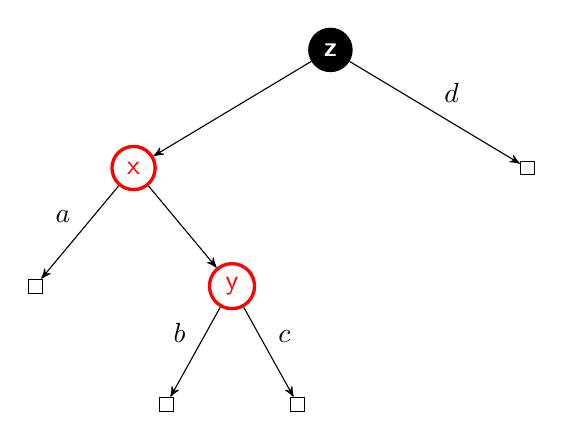
\begin{tikzpicture}[->,>=stealth',level/.style={sibling distance = 5cm/#1,level distance = 1.5cm}]
    \node [arn_n] {z}
        child{ node [arn_r] {x}
                child{ node [arn_x] {} edge from parent node[above left] {$a$}}
                child{ node [arn_r] {y}
                  child{ node [arn_x] {} edge from parent node[above left] {$b$}}
                  child{ node [arn_x] {} edge from parent node[above right] {$c$}}
                }
        }
        child{ node [arn_x] {} edge from parent node[above right] {$d$}}
    ;
    \end{tikzpicture}
    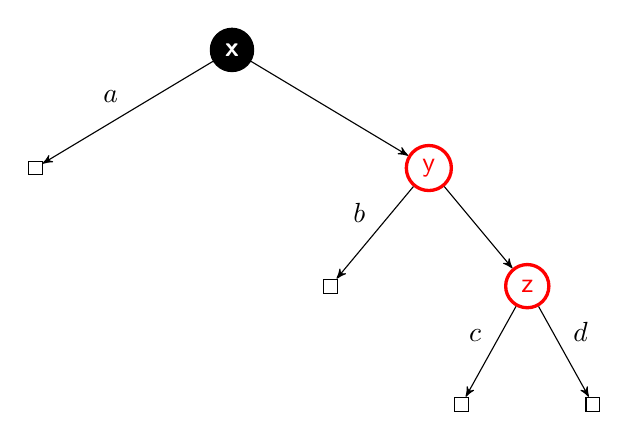
\begin{tikzpicture}[->,>=stealth',level/.style={sibling distance = 5cm/#1,level distance = 1.5cm}]
    \node [arn_n] {x}
        child{ node [arn_x] {} edge from parent node[above left] {$a$}}
        child{ node [arn_r] {y}
                child{ node [arn_x] {} edge from parent node[above left] {$b$}}
                child{ node [arn_r] {z}
                  child{ node [arn_x] {} edge from parent node[above left] {$c$}}
                  child{ node [arn_x] {} edge from parent node[above right] {$d$}}
                }
        }
    ;
    \end{tikzpicture}
    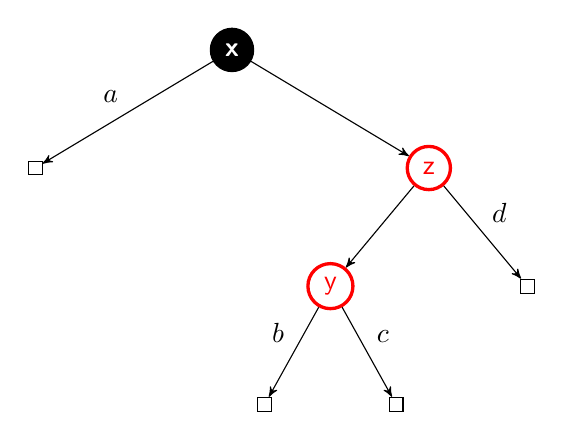
\begin{tikzpicture}[->,>=stealth',level/.style={sibling distance = 5cm/#1,level distance = 1.5cm}]
    \node [arn_n] {x}
        child{ node [arn_x] {} edge from parent node[above left] {$a$}}
        child{ node [arn_r] {z}
                child{ node [arn_r] {y}
                  child{ node [arn_x] {} edge from parent node[above left] {$b$}}
                  child{ node [arn_x] {} edge from parent node[above right] {$c$}}
                }
                child{ node [arn_x] {} edge from parent node[above right] {$d$}}
        }
    ;
    \end{tikzpicture}
\caption{Eliminating red nodes with red parents: before} \label{fig:violations}
\end{figure}

Figure \ref{fig:rebalance} displays the resulting subtree after the rebalance.

\begin{figure}
\centering
    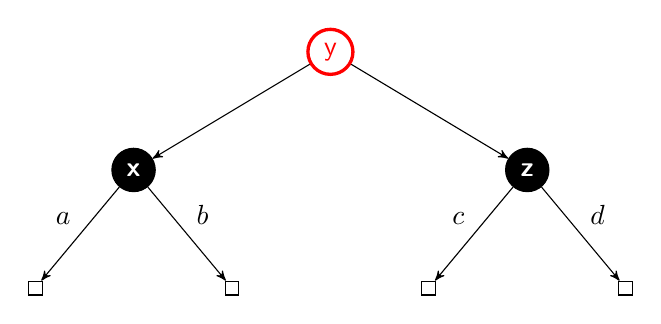
\begin{tikzpicture}[->,>=stealth',level/.style={sibling distance = 5cm/#1,level distance = 1.5cm}]
    \node [arn_r] {y}
        child{ node [arn_n] {x}
          child{ node [arn_x] {} edge from parent node[above left] {$a$}}
          child{ node [arn_x] {} edge from parent node[above right] {$b$}}
        }
        child{ node [arn_n] {z}
          child{ node [arn_x] {} edge from parent node[above left] {$c$}}
          child{ node [arn_x] {} edge from parent node[above right] {$d$}}
        }
    ;
    \end{tikzpicture}
\caption{Eliminating red nodes with red parents: after} \label{fig:rebalance}
\end{figure}

Here is the code of \code{insert}. You may notice that \code{balance} method is split in two different cases. This is an optimization because some cases are not possible depending on the branch you came for.

\begin{listing}[H]
  \begin{minted}[xleftmargin=20pt,linenos]{haskell}
insert
  :: (Ord a)
  => a -> RedBlackTree a -> RedBlackTree a
insert x tree =
  let (Bin _ a y b) = ins tree
  in Bin B a y b
    where
      ins               Tip  = Bin R Tip x Tip
      ins node@(Bin c a y b) =
        if      x < y   then lbalance (Bin c (ins a) y b)
        else if x > y   then rbalance (Bin c a y (ins b))
        else                 node

lbalance :: RedBlackTree a -> RedBlackTree a
lbalance (Bin B (Bin R (Bin R a x b) y c) z d) =
    Bin R (Bin B a x b) y (Bin B c z d)
lbalance (Bin B (Bin R a x (Bin R b y c)) z d) =
    Bin R (Bin B a x b) y (Bin B c z d)
lbalance tree                                  =
    tree

rbalance :: RedBlackTree a -> RedBlackTree a
rbalance (Bin B a x (Bin R b y (Bin R c z d))) =
    Bin R (Bin B a x b) y (Bin B c z d)
rbalance (Bin B a x (Bin R (Bin R b y c) z d)) =
    Bin R (Bin B a x b) y (Bin B c z d)
rbalance tree                                  =
    tree
  \end{minted}
  \caption{Red-black tree insert method}
  \label{lst:insert}
\end{listing}

Finally, the listing \ref{lst:fromOrdList} contains the code for the list constructor of a red-black tree.

The code is quite advance but it is basically taking advantage of the fact that we know the position of the node in the given tree, because the precondition of this method is that the given list is ordered, so we can remove the cost of searching the position of the $i$-th for each $i$ element inserted.

The total cost in time and space of this algorithm is $\mathcal{O}(n)$.

\begin{listing}[H]
  \begin{minted}[xleftmargin=20pt,linenos]{haskell}
fromOrdList :: [a] -> RedBlackTree a
fromOrdList xs' =
  toTree (Tip, ins ([], xs'))
    where
      balance' [(R, v1, t1)] = [(B, v1, t1)]
      balance' ((R, v1, t1):(R, v2, t2):(B, v3, t3):xs) =
        (B, v1, t1):(balance' ((R, v2, (Bin B t3 v3 t2)):xs))
      balance' xs = xs

      ins (ts, [])   = ts
      ins (ts, x:xs) = ins ( balance' ((R, x, Tip):ts), xs)

      toTree (t, [])                  =
        t
      toTree (t, ((color, v, t'):ts)) =
        toTree ((Bin color t' v t), ts)
  \end{minted}
  \caption{Red-black tree fromOrdList method}
  \label{lst:fromOrdList}
\end{listing}

\subsection{Documentation}\label{ss:documentation}

One cool feature of \textbf{cabal} \cite{cabal}, one of the most used building tool in Haskell, is that it can generate documentation \textit{"for free"} of your source code. Underneath, Cabal is using \textbf{haddock} \cite{haddock}, that can automatically generate documentation from annotated Haskell source code.

Haddock can generate documentation for a myriad of formats including \textit{html} and \textit{latex}. The documentation can be generated by \mint{bash}|$ cabal haddock|Here you can find a screenshot from the generated documentation from {\fontfamily{qcr}\selectfont RedBlackTree.hs}

\begin{figure}[H]
  \includegraphics[width=\textwidth]{haddock1}
  \centering
\end{figure}

\section{Experimentation}\label{s:experimentation}


Theoretically, the maximum depth of the tree is $2\lfloor \log (n+1) \rfloor$. Let's test if that fact holds in practice.

Before testing the maximum depth property of the red-black trees, we need to test the correctes of our code.

For this purpose, I created the following tests at \code{test/Chapter3/RedBlackTreeSpec.hs}

\begin{listing}[H]
  \begin{minted}[xleftmargin=1pt,linenos]{haskell}
spec :: Spec
spec = do
  describe "Red-black tree" $ do
    it "checkInvariants should check if
          invariants are fulfilled" $ do
      RBT.checkInvariants rbt1 `shouldBe` True
      RBT.checkInvariants bad  `shouldBe` False
      RBT.checkInvariants bad2 `shouldBe` False

    it "insert should preserve invariants" $ do
      let rbt = foldr RBT.insert
                      RBT.empty
                      ([1..10000] :: [Int])
      RBT.checkInvariants rbt `shouldBe` True

    it "fromOrdList should preserve invariants" $ do
      let rbt = RBT.fromOrdList [1..10000] :: RedBlackTree Int
      RBT.checkInvariants rbt `shouldBe` True

    it "toOrdList should return an ordered list of the
          elements of the tree" $ do
      let rbt = foldr RBT.insert
                      RBT.empty
                      ([3,5,2,1,8,9,5,4] :: [Int])
      RBT.toOrdList rbt `shouldBe` [1,2,3,4,5,8,9]

    it "toOrdList . fromOrdList == id" $ do
      let xs = [1..1000] :: [Int]
          f = RBT.toOrdList . RBT.fromOrdList
      f xs `shouldBe` xs

    prop "maxDepth = 2*floor[log (n + 1)]" $ do
      property $
        \(n :: Positive Int) ->
           let size = 1000
               rbt = RBT.fromOrdList [1..size]
           in RBT.maxDepth rbt
                <= 2*floor (logBase 2.0 (fromIntegral size + 1.0))
  \end{minted}
  \caption{Red-black tree fromOrdList method}
  \label{lst:fromOrdList}
\end{listing}

In order to prove the maximum depth property of the red-black trees we are going to implement the following experiment:

\begin{enumerate}
  \item Generate $n$ randomly-built red-black trees of size $m$, where $n$ and $m$ are large enough.
  \item Compute the height of the $n$ red-black trees.
  \item Compute the max, mean and standard deviation of the depth of each red-black tree.
  \item Compare it to the theoretically maximum heigth.
\end{enumerate}

The haskell code to generate the randomly-built red-black tree of size $m$ uses a property-based testing library called QuickCheck \cite{quickcheck} that allows the user to generate a huge amount of uniformly distributed random data.

\begin{listing}[H]
  \begin{minted}[xleftmargin=10pt,linenos]{haskell}

-- | A generator for values of type 'RedBlackTree' of the given size.
genRBT :: (Arbitrary a, Ord a)
       => Int -> Gen (RedBlackTree a)
genRBT = fmap (fromList . unUnique) . genUniqueList

newtype UniqueList a = UniqueList { unUnique :: [a] }
    deriving Show

-- | 90 % of samples are randomly distributed elements
--   10 % are sorted.
genUniqueList :: (Arbitrary a, Ord a)
              => Int -> Gen (UniqueList a)
genUniqueList n =
  frequency [ (9, genUniqueList' n arbitrary)
            , (1, (UniqueList . unSorted) <$>
                    genUniqueSortedList n arbitrary)
            ]

genUniqueList' :: (Eq a) => Int -> Gen a -> Gen (UniqueList a)
genUniqueList' n gen =
  UniqueList <$> vectorOf n gen `suchThat` isUnique

newtype UniqueSortedList a =
    UniqueSortedList { unSorted :: [a] }
  deriving Show

genUniqueSortedList :: (Ord a)
                    => Int -> Gen a -> Gen (UniqueSortedList a)
genUniqueSortedList n gen =
  UniqueSortedList . List.sort . unUnique <$> genUniqueList' n gen

isUnique :: Eq a => [a] -> Bool
isUnique x = List.nub x == x

  \end{minted}
  \caption{QuickCheck generators.}
  \label{lst:quickcheck}
\end{listing}

The code of the experiment is the following

\begin{listing}[H]
  \begin{minted}[xleftmargin=10pt,linenos]{haskell}
-- 1.- Generate a random vector of [n-m, n+m] elements
-- 2.- Transform it into a red-black tree.
-- 3.- Compute the maximum length
-- 4.- Get the statistics
-- 5.- Output them on the stdout
runExperiment
  :: Int -- ^ Number of samples
  -> Int -- ^ Size of the samples
  -> IO ()
runExperiment n size = do
  samples <- generate $ replicateM n (RBT.genRBT @Int size)
  let (Just max', mean, std) =
    L.fold ((,,) <$> L.maximum <*> L.mean <*> L.std) $
                        fmap (fromIntegral . RBT.maxDepth) samples
  report n size max' mean std

  \end{minted}
  \caption{Experiment of the theoretical depth of a red-black tree.}
  \label{lst:experiment}
\end{listing}

\begin{listing}[H]
  \begin{minted}[xleftmargin=1pt,linenos]{haskell}
# samples: 100
tree size: 100

max depth(max) : 8.0
max depth(mean): 7.720000000000001
max depth(std) : 0.448998886412873

max depth  (theoretical): 12
perfectly balanced depth: 6
  \end{minted}
  \caption{Output of the experiment for 100 samples of size 100.}
  \label{lst:output}
\end{listing}

From the output of the experiment, we conclude that the theorical maximum depth holds for an empirical red-black tree. Furthemore, the height is near to a perfectly balanced binary tree.

\section{Conclusion}\label{s:conclusion}

We have coded a simple, yet efficient purely functional implementation of red-black trees in Haskell and have proved that the maximum theoretical depth holds in practice by conducting an empirical experiment over randomly generated red-black trees.

\section{Curiosity}\label{s:curiosity}

One of the reasons this implementation is so much  simpler than typical presentations of red-black trees (e.g., Chapter 14 of \cite{clr90}) is that it uses subtly different  rebalancing  transformations.  Imperative implementations typically split the four dangerous cases considered here into eight cases, according to the color  of the sibling  of the red node with a red child.  Knowing the color of the red parent's  sibling allows the transformations  to use fewer  assignments in some cases and to terminate rebalancing early in others.

However, in a functional setting, where we are copying the nodes in question  anyway, we cannot reduce the number  of assignments in this fashion, nor can we terminate copying early, so there is no point is using the more complicated transformations.

%%%%%%%%%%%%%%%% Appendix %%%%%%%%%%%%%%%%%%%%%

\newpage

\section*{Appendix A}\label{s:appendix-a}

\subsection*{RedBlackTree.hs}\label{s:redblacktree}

\inputminted{haskell}{../../Chapter3/RedBlackTree.hs}

%%%%%%%%%%%%%%%% BIBLIOGRAPHY %%%%%%%%%%%%%%%%%%%%%

\bibliographystyle{alpha}
\bibliography{refs}

%%%%%%%%%%%%%%%%%%%%%%%%%%%%%%%%%%%%%%%%%%%%%%%%%%%%%

\end{document}
